% !TEX root = univariate.tex

UnivariePour commencer, ce rapport comportera une analyse univariée de chacune des variables quantitatives et qualitatives qui font partie de le jeu de données, en suite il passera a l'analyse bivariée pour vérifier des liens entre les variables quantitatives mesurées par la corrélation linéaire.

\begin{figure}
    \centering
    \subfloat[le 90 \%  du échantillon ont moins des 200 hits dans la session ou ils ont effectué au moins une transaction.]{
        \label{hits}
        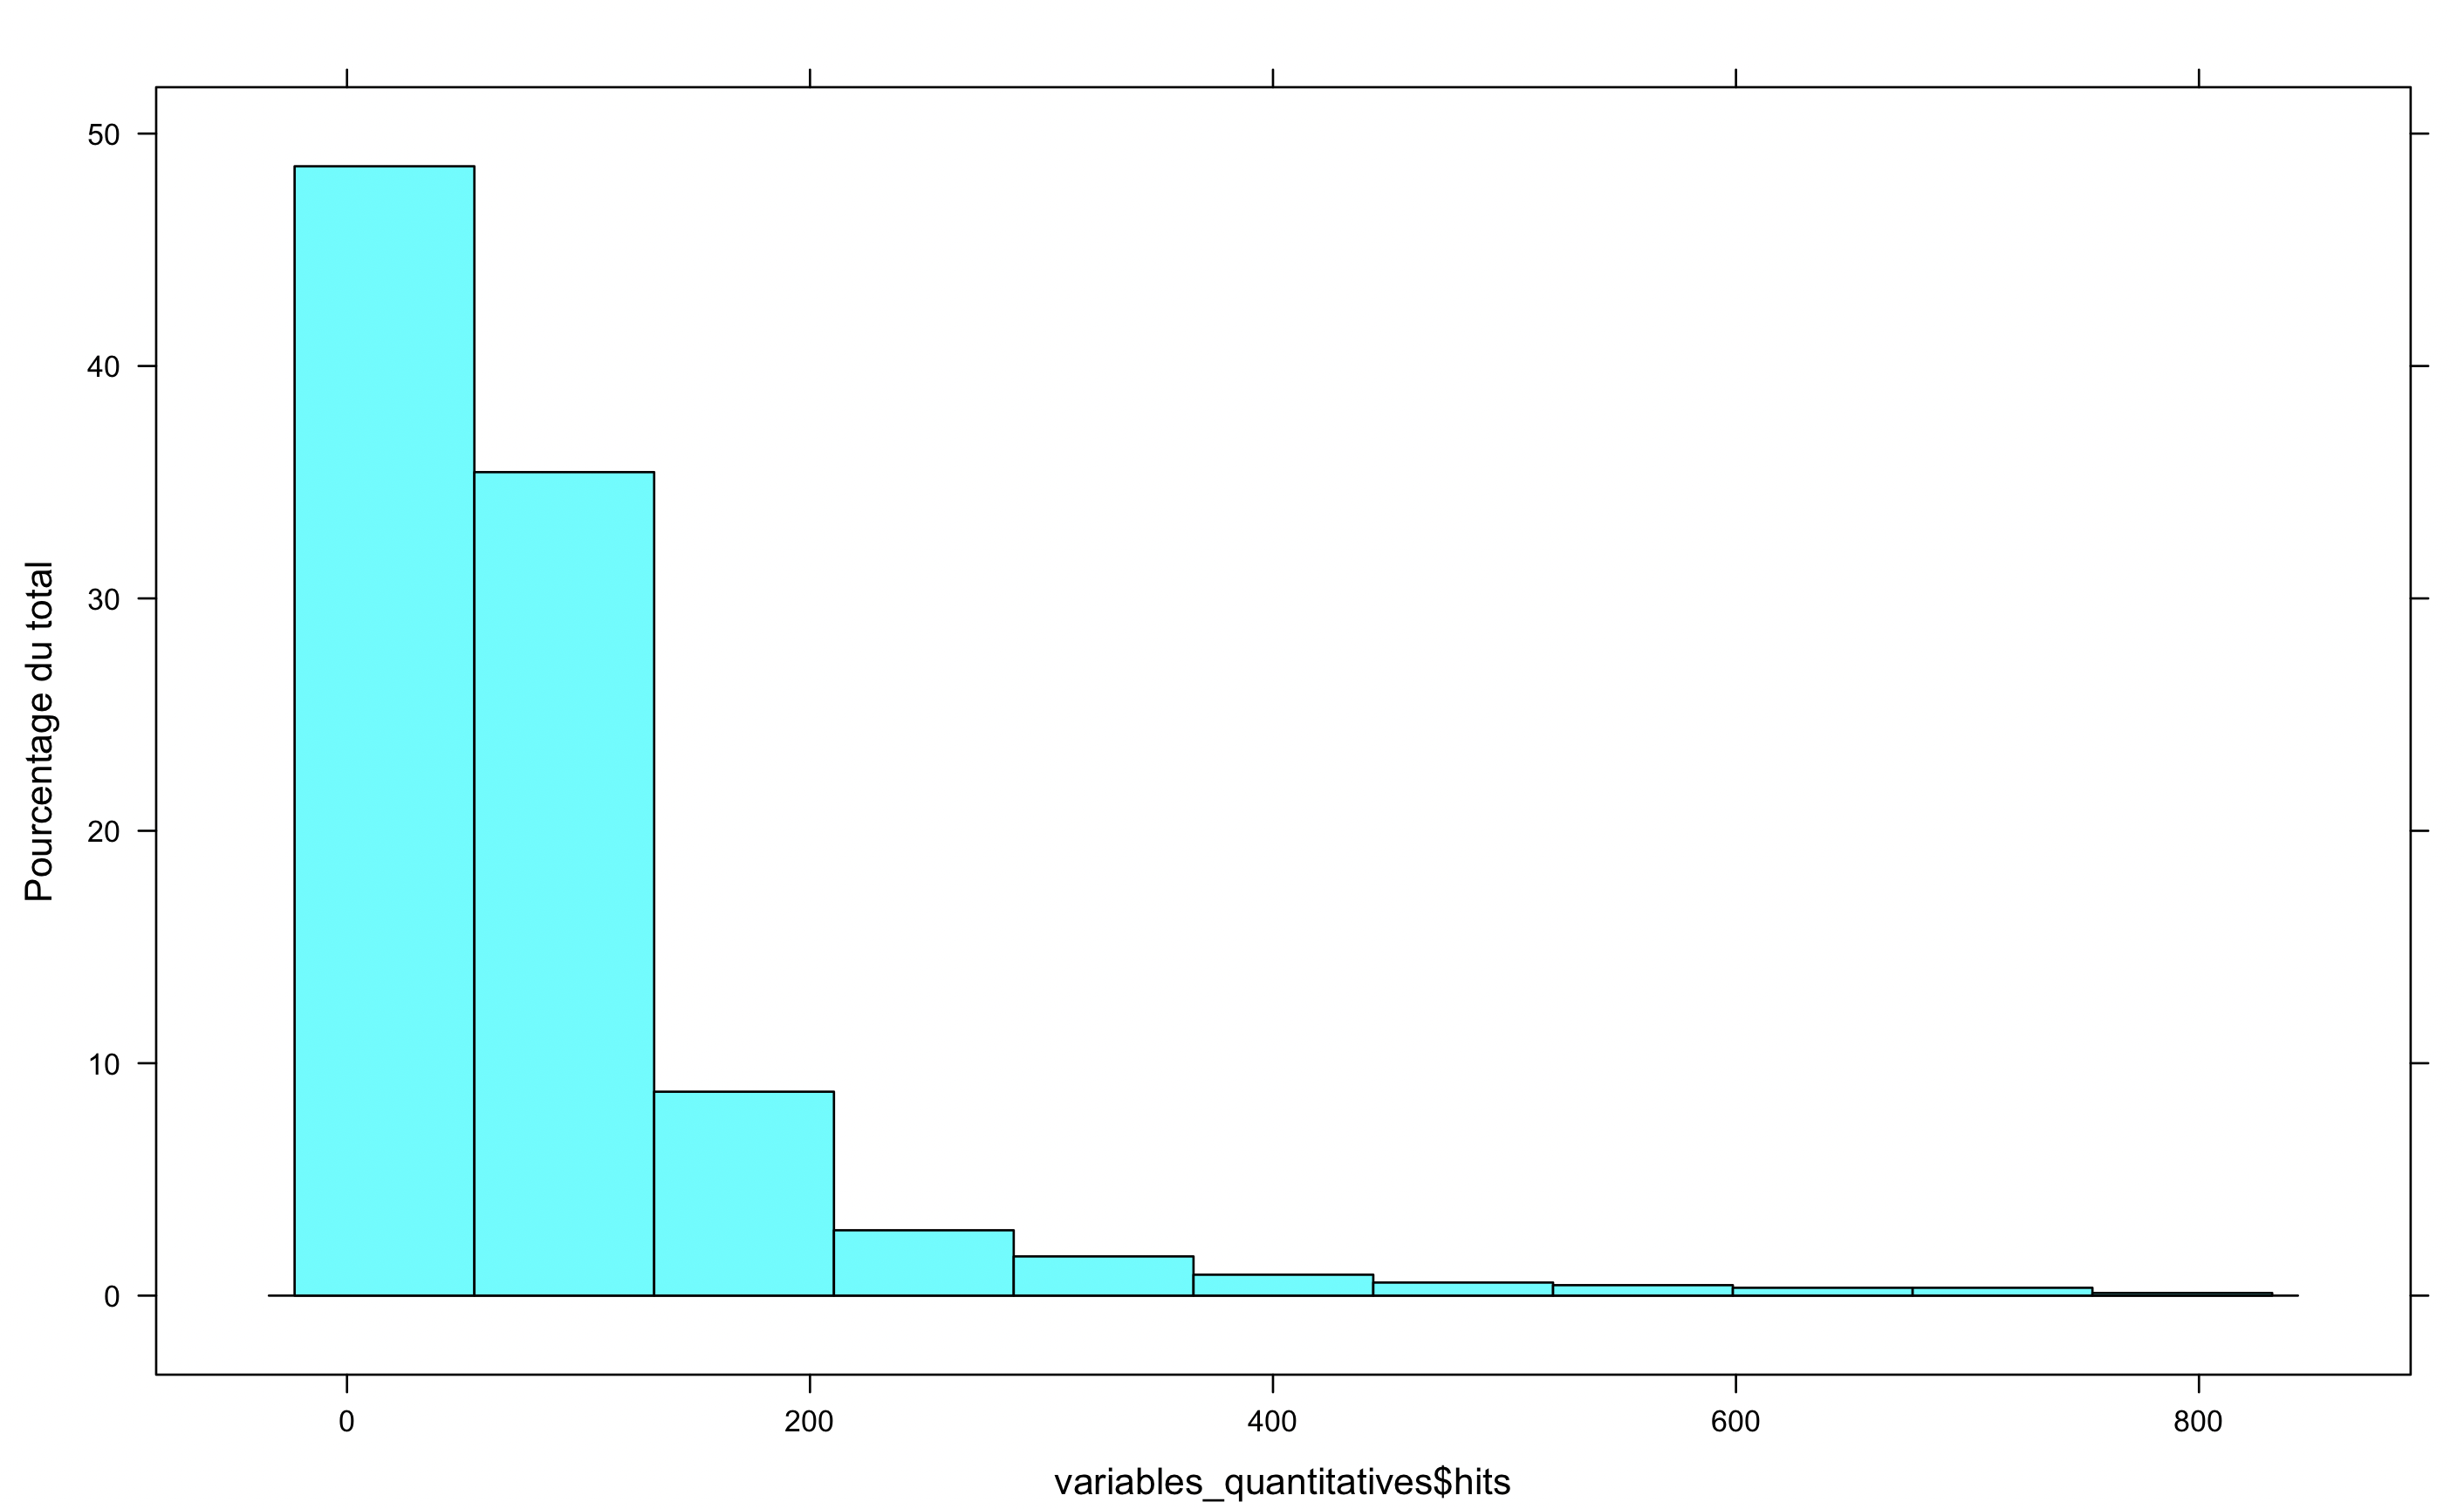
\includegraphics[width=0.45\textwidth]{scriptsR/imgs/univarie/hits_percent.png}
    }
    \hfill
    \subfloat[Le 70 \% des transactions ont été réalisées par des nouveaux utilisateurs.]{
        \label{new_visit}
        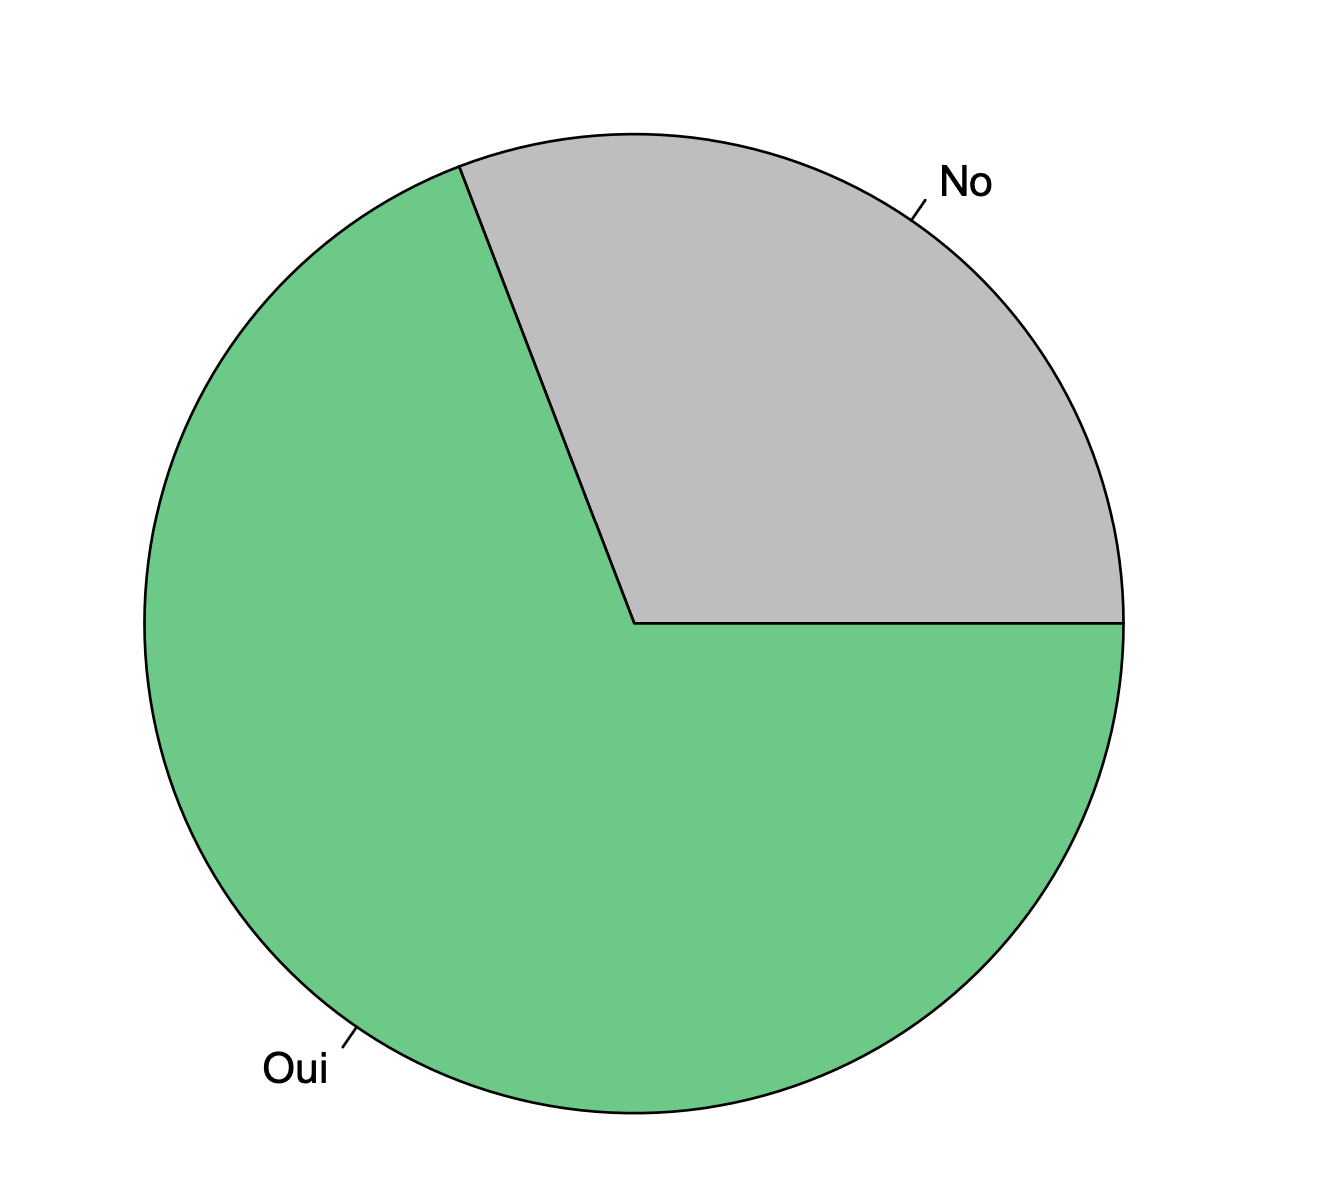
\includegraphics[width=0.45\textwidth]{scriptsR/imgs/univarie/newVisit.png}
    }
     \hfill
    \subfloat[Pour page views, Nous avons quelques valeurs atypiques qu'on veut supprimer avant de passer a l'étape suivant. Le 80 \%  du échantillon ont entre 0 et 25 pages vues.]{
        \label{page_views}
        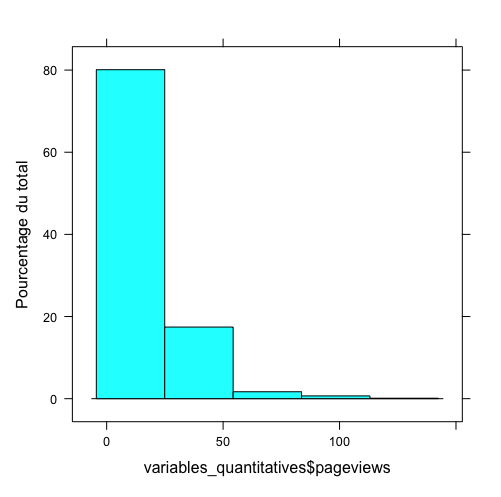
\includegraphics[width=0.45\textwidth]{scriptsR/imgs/univarie/pageviews.png}
    }
    \hfill
    \subfloat[La majorité de transactions sont entrées 0\euro  et  100\euro , Nous avons aussi des transactions atypiques qui  arrivent jusqu'à 800\euro ]{
        \label{transaction_revenue}
        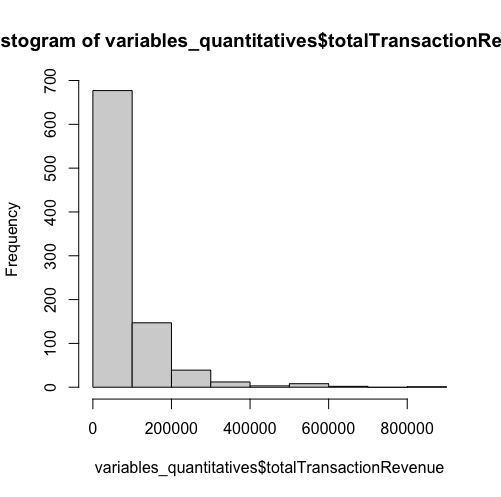
\includegraphics[width=0.45\textwidth]{scriptsR/imgs/univarie/transactionsrevenue.png}
    }
    \hfill
    \subfloat[La majorité des individus font 1 transaction dans la session, ce qui correspond à la quantité attendu.]{
        \label{transactions}
        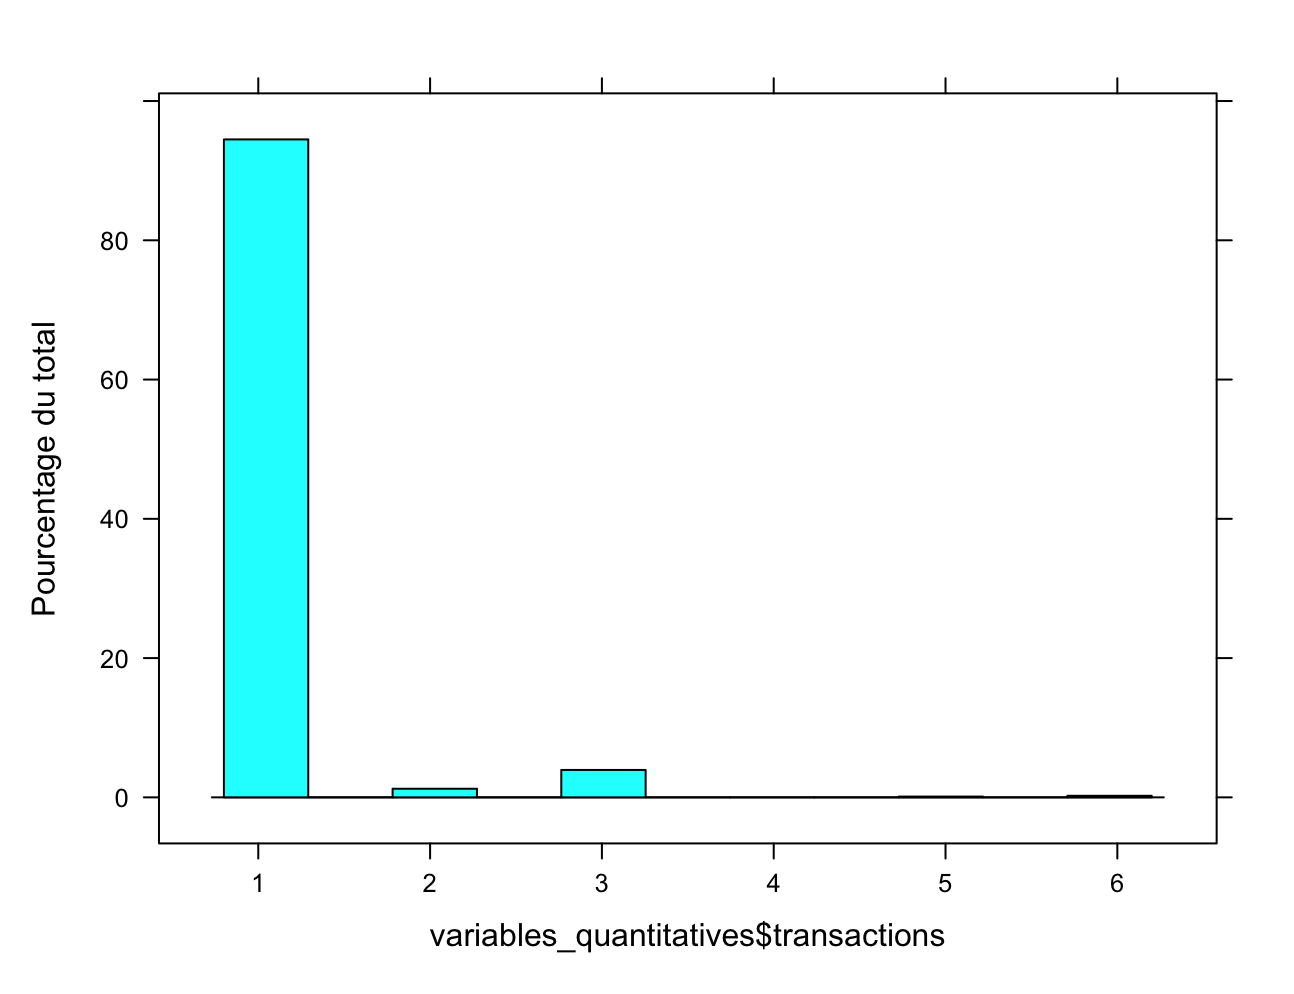
\includegraphics[width=0.45\textwidth]{scriptsR/imgs/univarie/transactionsHistogram.png}
    }
    \hfill
    \subfloat[Les individus prennent moins d'un minute pour effectuer au moins une transaction, le plus part entre eux, prennent moins des 20 secondes.]{
        \label{timeOnSite}
        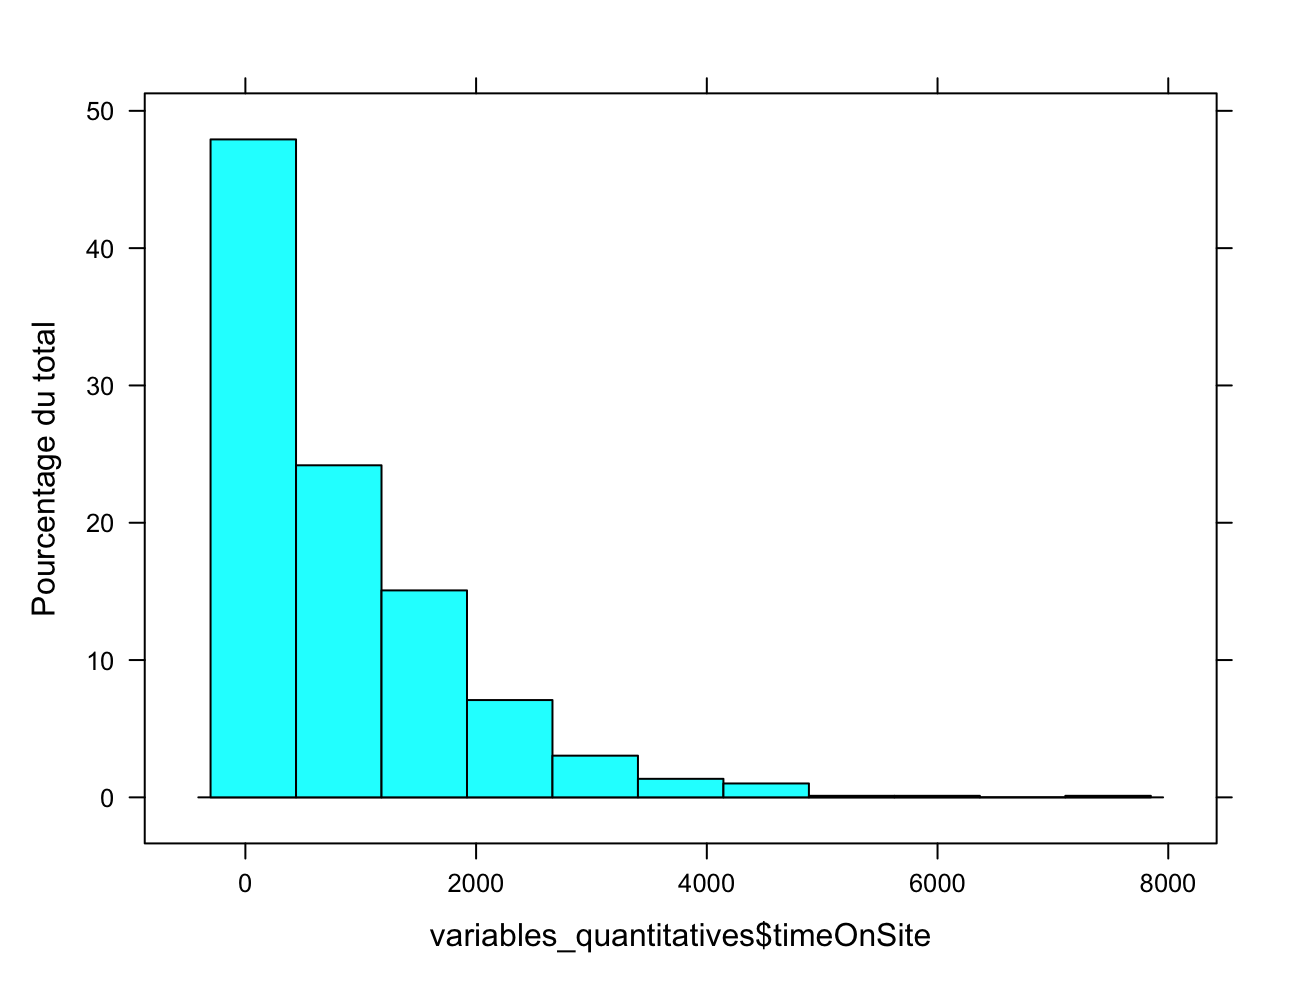
\includegraphics[width=0.45\textwidth]{scriptsR/imgs/univarie/TimeOnSIteHist.png}
    }

     
    \caption{Overall caption}
    \label{ref_label_overall}
\end{figure}


\begin{figure}
\ContinuedFloat
    \centering

    \subfloat[Chrome est le navigateur préféré des utilisateurs du échantillon suivi par safari, suivi de la version mobile de chrome.]{
        \label{browserName}
        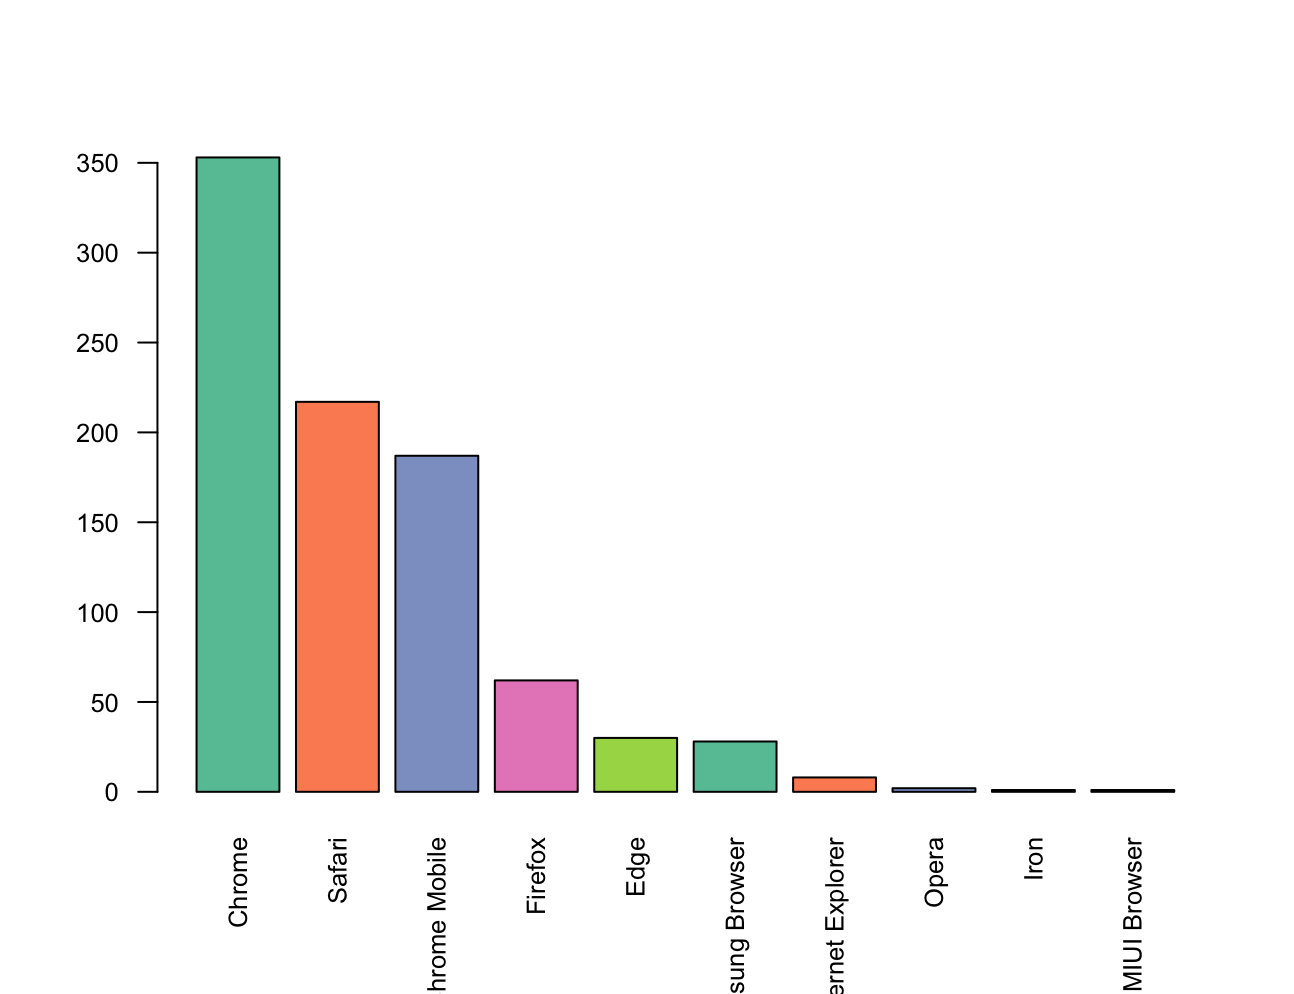
\includegraphics[width=0.45\textwidth]{scriptsR/imgs/univarie/browser_name.png}
    }
    \hfill
    \subfloat[Il existe un pourcentage important d'individus qui ont effectué une transaction à partir d'un écran dont la largeur est inférieure à 500, nous pouvons en déduire qu'ils ont été réalisés depuis un appareil mobile,  suivi d'une autre plage comprise entre 1800 et 190.]{
        \label{browser_widthBoxplot}
        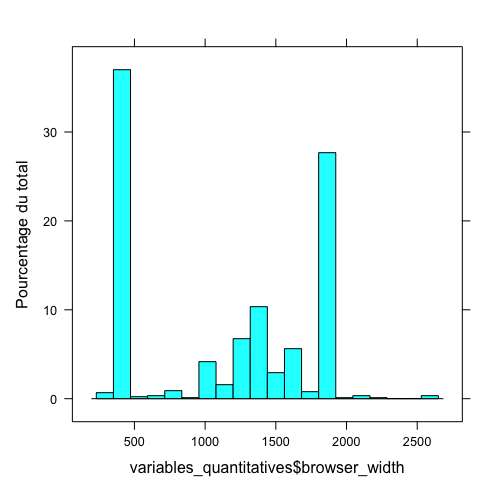
\includegraphics[width=0.45\textwidth]{scriptsR/imgs/univarie/browser_width.png}
    }
    \hfill
    \subfloat[les données sont distribuées d'une manière plus uniforme, nous remarquons que les plus part de largeur d'écrans sont entre 600 pixels et 1000 pixels, nous n'observons pas de données exceptionnels ]{
        \label{browser_heightBoxplot}
        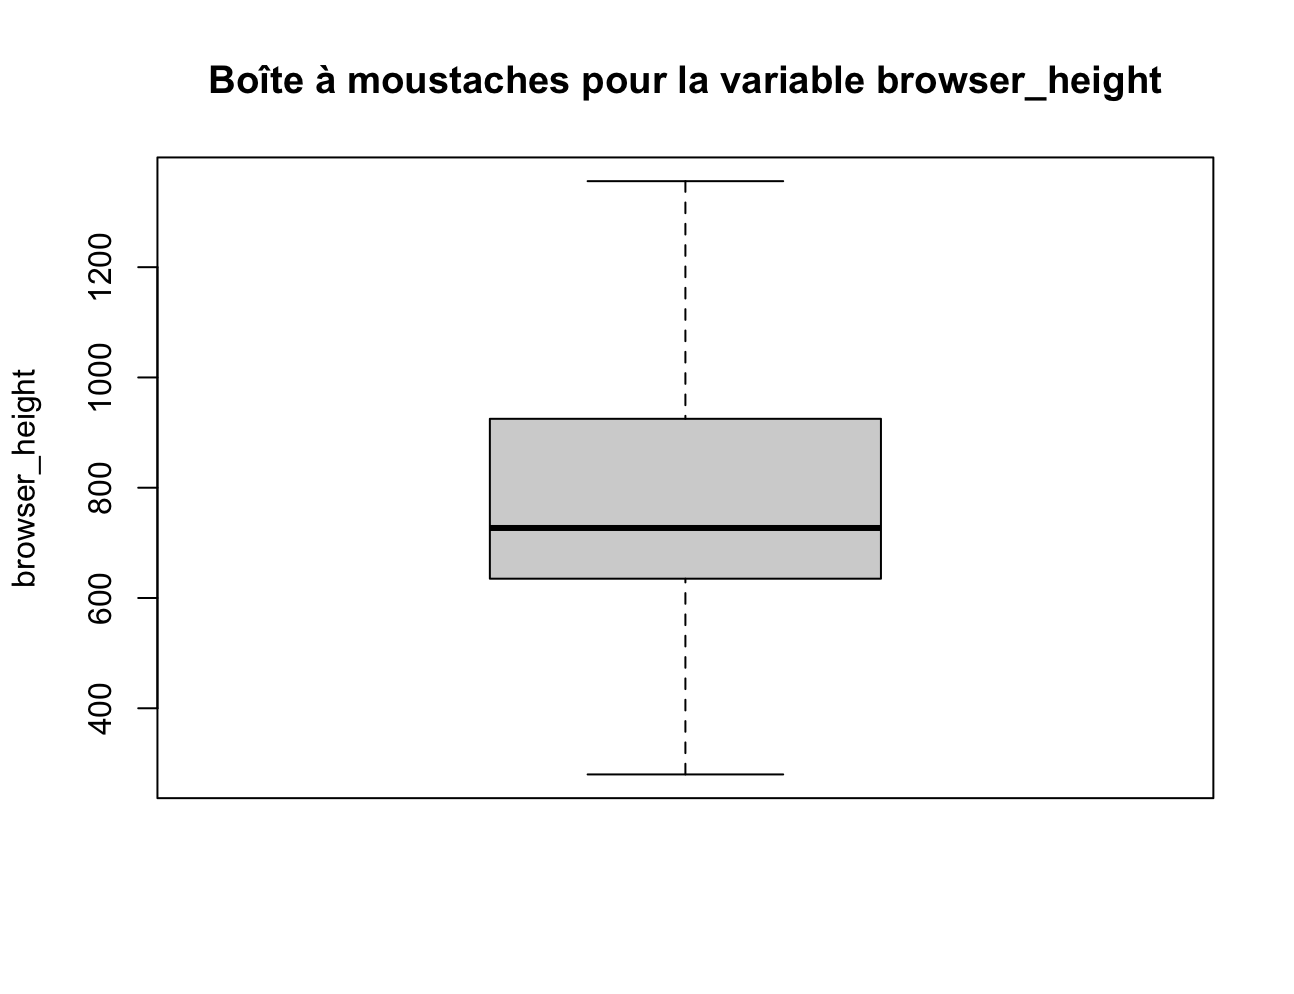
\includegraphics[width=0.45\textwidth]{scriptsR/imgs/univarie/browser_height_bloxplot.png}
    }
    \hfill
    \subfloat[Contrairement a ce que nous avons constaté avec autres variables, les 57 \% des transactions ont étés réalisé depuis une laptop, suivi d'un 38\%  avec un dispositif mobile.]{
        \label{deviceCategory}
        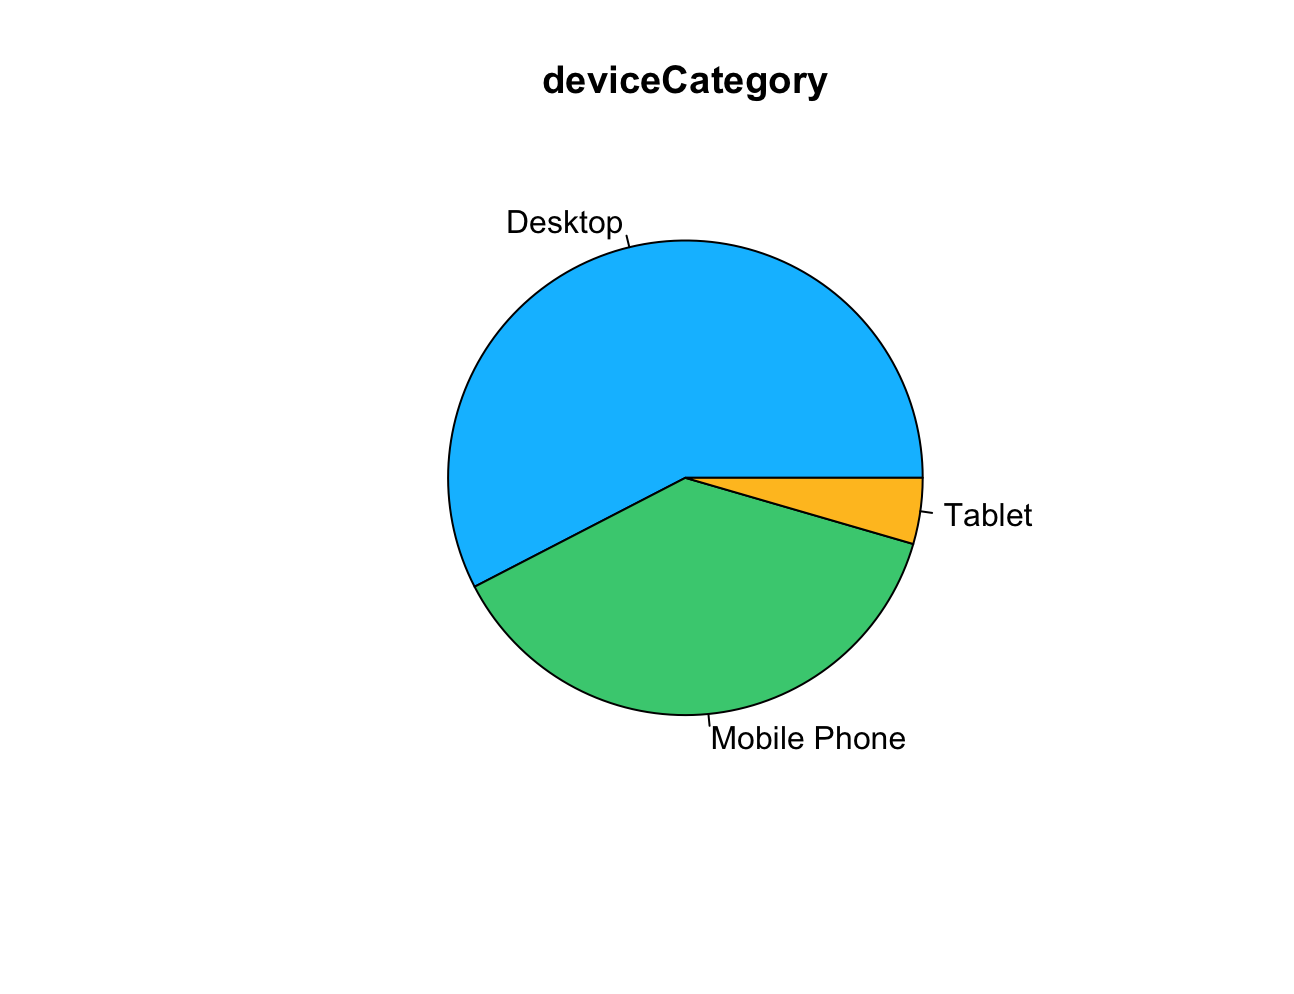
\includegraphics[width=0.45\textwidth]{scriptsR/imgs/univarie/deviceCategory.png}
    }
    \hfill
    \subfloat[Windows 10 est le système d'exploitation préféré du échantillon. ]{
        \label{operatingSys}
        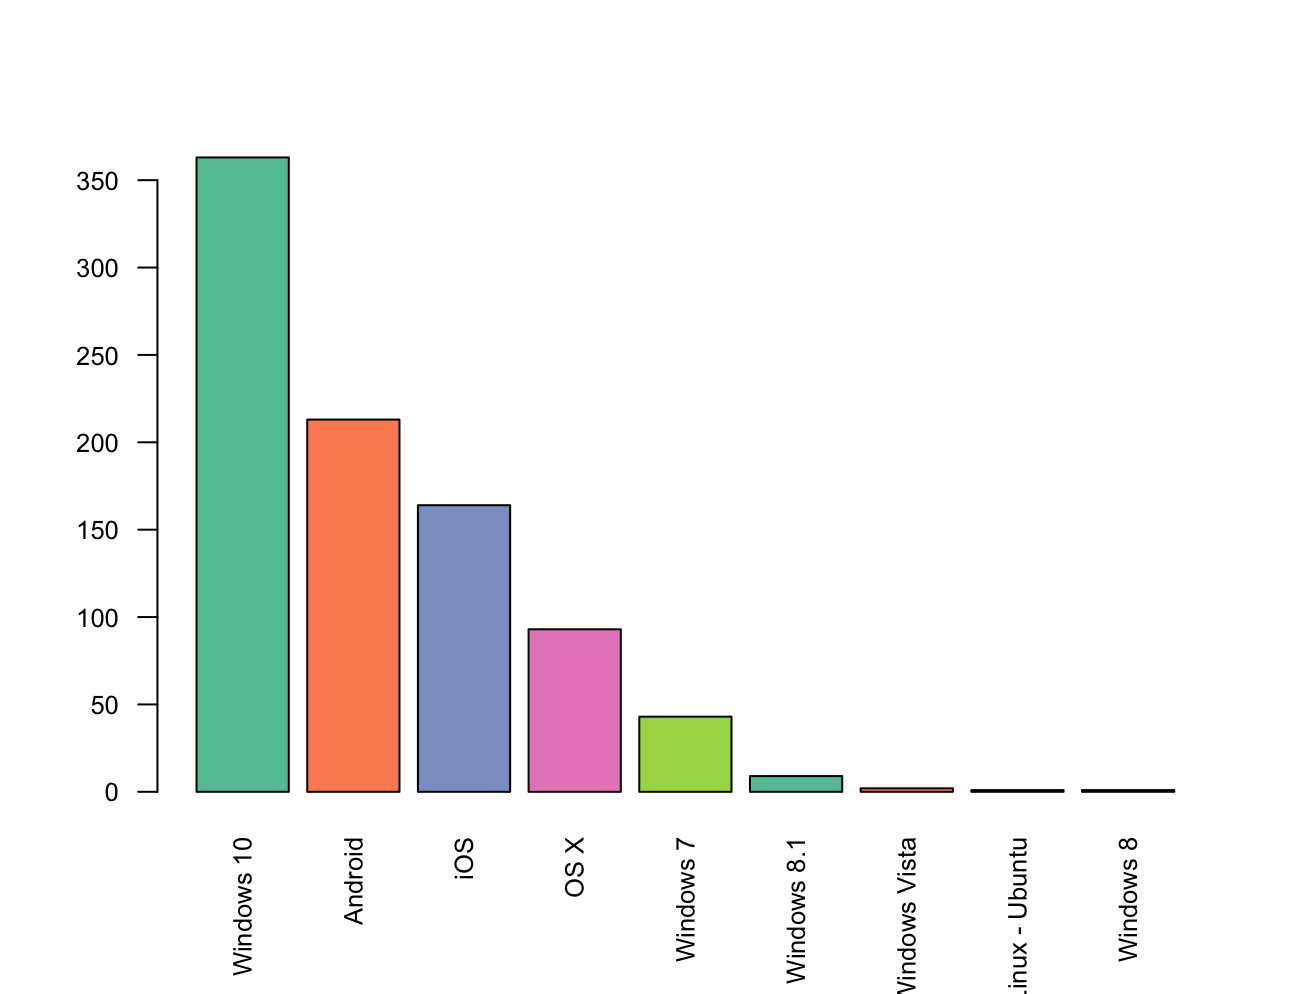
\includegraphics[width=0.45\textwidth]{scriptsR/imgs/univarie/operatingSys.png}
    }
    \hfill
    \subfloat[L'anglais américain et le français du France sont les langues préférées des utilisateurs lorsqu'ils effectuent une transaction.]{
        \label{language}
        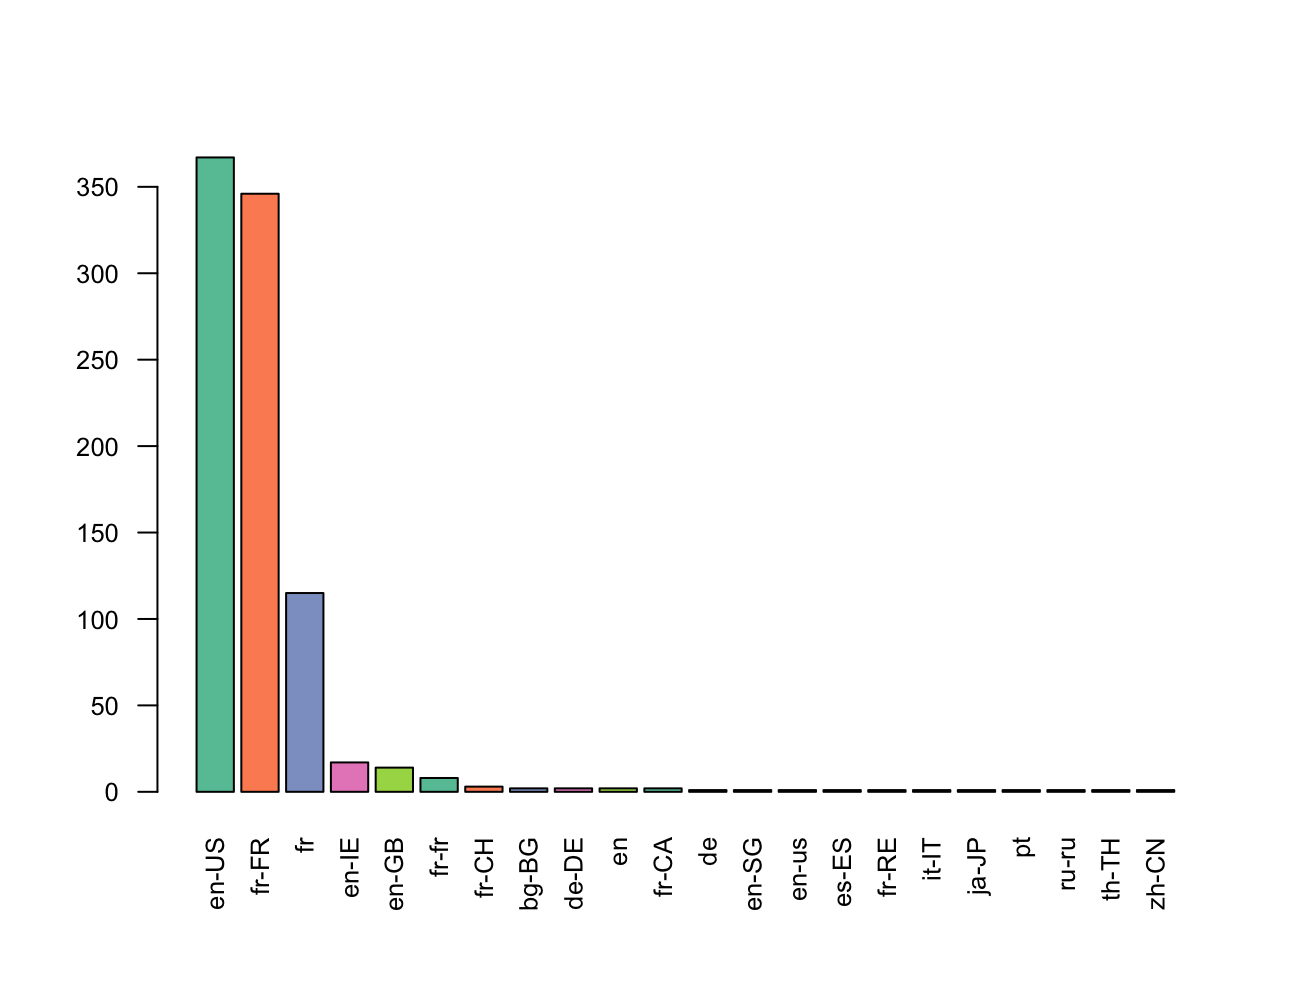
\includegraphics[width=0.45\textwidth]{scriptsR/imgs/univarie/language.png}
    }

    \caption{Overall caption2}
    \label{ref_label_overall}
\end{figure}


\begin{figure}
\ContinuedFloat
    \centering

      \subfloat[Avec plus de 600 sessions, la carte de crédit est le mode de paiement le plus utilisé pour les transats, suivi de Paypal avec un peu plus de 100 session. ]{
        \label{paymentMethod}
        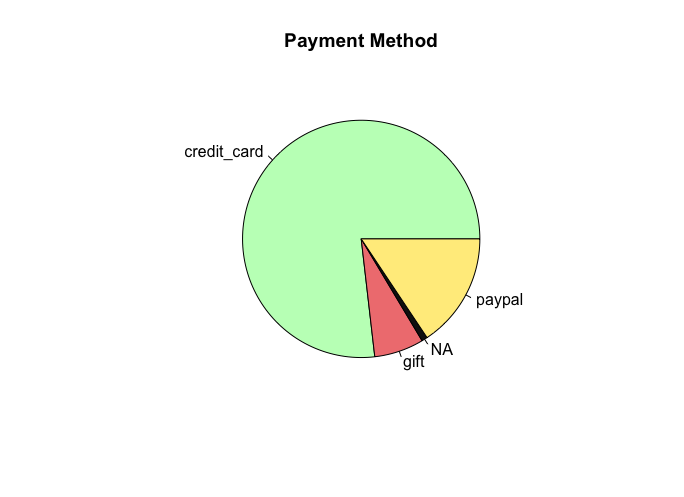
\includegraphics[width=0.45\textwidth]{scriptsR/imgs/univarie/paymentMethod.png}
    }
    \hfill
    \subfloat[Dans un peu plus de la moitié des sessions, les transactions effectuées comprenaient 1, 2 ou 3 articles, mais un nombre important de transactions contenaient entre 5 et 10 articles. ]{
        \label{itemcountHistogram}
        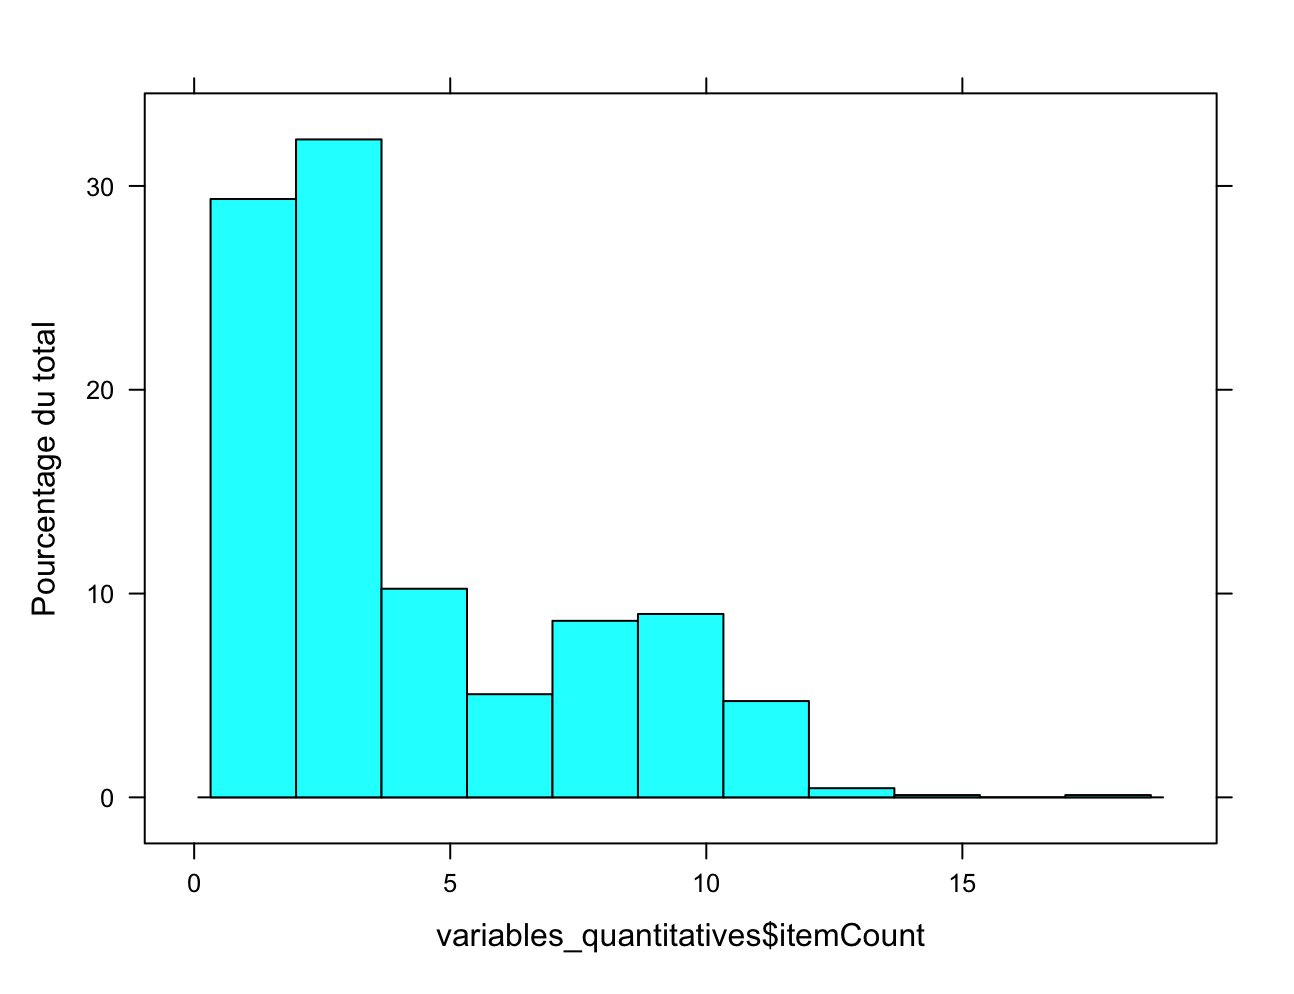
\includegraphics[width=0.45\textwidth]{scriptsR/imgs/univarie/itemcountHistogram.png}
    }
    \caption{Overall caption3}
    \label{ref_label_overall}
\end{figure}





